% !TEX program = pdflatex
% !TEX options = -synctex=1 -interaction=nonstopmode -file-line-error "%DOC%"
% 固体物理第五次作业
\documentclass[UTF8,10pt,a4paper]{article}
\usepackage{ctex}
% \catcode`\。=\active
% \newcommand{。}{.}
\newcommand{\CourseName}{固体物理}
\newcommand{\CourseCode}{PHYS1502}
\newcommand{\Semester}{2019-2020学年第二学期}
\newcommand{\ProjectName}{第五次作业}
\newcommand{\DueTimeType}{截止时间}
\newcommand{\DueTime}{2020. 4. 10(周五)17:00}
\newcommand{\StudentName}{陈稼霖}
\newcommand{\StudentID}{45875852}
\usepackage[vmargin=1in,hmargin=.5in]{geometry}
\usepackage{fancyhdr}
\usepackage{lastpage}
\usepackage{calc}
\pagestyle{fancy}
\fancyhf{}
\fancyhead[L]{\CourseName}
\fancyhead[C]{\ProjectName}
\fancyhead[R]{\StudentName}
\fancyfoot[R]{\thepage\ / \pageref{LastPage}}
\setlength\headheight{12pt}
\fancypagestyle{FirstPageStyle}{
    \fancyhf{}
    \fancyhead[L]{\CourseName\\
        \CourseCode\\
        \Semester}
    \fancyhead[C]{{\Huge\bfseries\ProjectName}\\
        \DueTimeType\ : \DueTime}
    \fancyhead[R]{姓名 : \makebox[\widthof{\StudentID}][s]{\StudentName}\\
        学号 : \StudentID\\
        成绩 : \underline{\makebox[\widthof{\StudentID}]{}}}
    \fancyfoot[R]{\thepage\ / \pageref{LastPage}}
    \setlength\headheight{36pt}
}
\usepackage{amsmath,amssymb,amsthm,bm}
\allowdisplaybreaks[4]
\newtheoremstyle{Problem}
{}
{}
{}
{}
{\bfseries}
{.}
{ }
{第\thmnumber{ #2}\thmname{ #1}\thmnote{ (#3)} 得分: \underline{\qquad\qquad}}
\theoremstyle{Problem}
\newtheorem{prob}{题}
\newtheoremstyle{Solution}
{}
{}
{}
{}
{\bfseries}
{:}
{ }
{\thmname{#1}}
\makeatletter
\def\@endtheorem{\qed\endtrivlist\@endpefalse}
\makeatother
\theoremstyle{Solution}
\newtheorem*{sol}{解}
\providecommand{\abs}[1]{\left\lvert#1\right\rvert}
\usepackage{graphicx}
\begin{document}
\thispagestyle{FirstPageStyle}
\begin{prob}[(8.1) Potential Between Atoms]
    As a model of thermal expansion, we study the distance between two nearest-neighbor atoms in an anharmonic potential that looks roughly like this
    \begin{figure}[h]
        \centering
        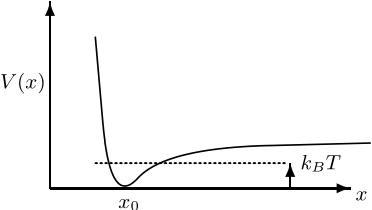
\includegraphics[width=.32\textwidth]{1.png}
    \end{figure}
    where $x$ is the distance between the two neighboring atoms. This potential can be expanded around its minimum as
    \[
        V(x)=\frac{\kappa}{2}(x-x_0)^2-\frac{\kappa}{3!}(x-x_0)^3+\cdots\tag{8.4}
    \]
    where the minimum is at position $x_0$ and $\kappa_3>0$. For small energies, we can truncate the series at the cubic term. (Note that we are defining the energy at the bottom of the well to be zero here.)\\
    A very accurate approximate form for interatomic potentials (particularly for inert atoms such as helium or argon) is given by the so-called Lennard-Jones potential
    \[
        V(x)=4\epsilon\left[\left(\frac{\sigma}{x}\right)^{12}-\left(\frac{\sigma}{x}\right)^6\right]+\epsilon\tag{8.5}
    \]
    where $\epsilon$ and $\sigma$ are constants that depend on the particular atoms we are considering.
    \begin{itemize}
        \item[$\triangleright$] What is the meaning of the exponent $6$ in the second term of the expansion (i.e., why is the exponent necessarily chosen to be $6$).
        \item[$\triangleright$] By expanding Eq. 8.5 around its minimum, and comparing to Eq. 8.4, calculate the values of the coefficients $x_0$, $\kappa$, and $\kappa_3$ for the Lennard-Jones potential in terms of the constants $\epsilon$ and $\sigma$. We will need these results in Exercise 8.3.
    \end{itemize}
\end{prob}
\begin{sol}
    \begin{itemize}
        \item[$\triangleright$] $6$次指数项代表着范德华力对应的势能,刻画了两个原子在远距离下的吸引效应,它的本质是电偶极相互作用.\\
        我们可以用一个简单的例子来推导这个六次指数项:考虑两个氢原子组成的系统(图\ref{1-1}),当其相距较远时,该系统的哈密顿是两个独立氢原子哈密顿的简单加和:
        \begin{equation}
            H_0=-\frac{\hbar^2}{2m}(\nabla_1^2+\nabla_2^2)-\frac{e^2}{4\pi\varepsilon_0r_1}-\frac{e^2}{4\pi\varepsilon_0r_2}.
        \end{equation}
        该系统的波函数为两个独立氢原子波函数的直积
        \begin{equation}
            \Psi=\psi_1(\bm{r}_1)\psi_2(\bm{r}_2)=\lvert n_1l_1m_1\rangle\lvert n_2l_2m_2\rangle.
        \end{equation}
        该系统的基态为$\lvert 100\rangle\lvert 100\rangle$.
        \begin{figure}[h]
            \centering
            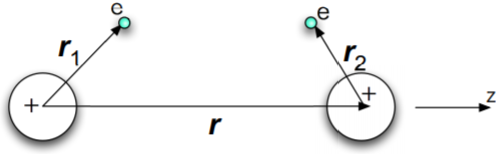
\includegraphics[width=.32\textwidth]{1-1.png}
            \caption{两个氢原子组成的系统. 设电子质量为$m$,电量为$-e$,原子核电量$+e$,两个原子核沿$z$轴排列,相距$r$,第一个原子核到其电子的距离为$r_1$,第二个原子核到其电子的距离为$r_2$.}
            \label{1-1}
        \end{figure}
        \\当两个氢原子靠近,则两者间发生相互偶极作用,将相互作用对应的库仑势能视为系统哈密顿的微扰项:
        \begin{equation}
            V=\frac{e^2}{4\pi\varepsilon_0r}-\frac{e^2}{4\pi\varepsilon_0}\frac{1}{\abs{-\bm{r}_1+\bm{r}_2}}-\frac{e^2}{4\pi\varepsilon_0}\frac{1}{\abs{\bm{r}+\bm{r}_2}}+\frac{e^2}{4\pi\varepsilon_0}\frac{1}{\abs{-\bm{r_1}+\bm{r}+\bm{r}_2}}.
        \end{equation}
        假设两个原子核间的距离远大于各个原子核与其电子间的距离,即$r\gg r_1,r_2$,利用展开式$(1+x)^{-1/2}=1-x^2/2+3x^2/8+\cdots$,我们有如下近似
        \begin{align}
            \nonumber\abs{\bm{r}-\bm{r}_1}=&[(x-x_1)^2+(0-y_1)^2+(0-z_1)^2]^{-1/2}=r^{-1}\left[\frac{z^2-2zz_1+x_1^2+y_1^2+z_1^2}{r^2}\right]^{-1/2}\\
            =&r^{-1}\left[1+\frac{-2zz_1+x_1^2+y_1^2+z_1^2}{r^2}\right]^{-1/2}\approx r^{-1}\left(1-\frac{-2zz_1+x_1^2+y_1^2+z_1^2}{2r^2}+\frac{3z_1^2}{2r^2}\right),\\
            \abs{\bm{r}+\bm{r}_2}^{-1}\approx&r^{-1}\left(1-\frac{2zz_2+x_2^2+y_2^2+z_2^2}{2r^2}+\frac{3z_2^2}{2r^2}\right),\\
            \abs{\bm{r}-\bm{r}_1+\bm{r}_2}^{-1}\approx&r^{-1}\left[1-\frac{-2zz_1+2zz_2+x_1^2-2x_1x_2+x_2^2+y_1^2-2y_1y_2+y_2^2+z_1^2-2z_1z_2+z_2^2}{2r^2}+\frac{3(z_2-z_1)^2}{r^2}\right].
        \end{align}
        故微扰项可近似为
        \begin{align}
            \nonumber V\approx&\frac{e^2}{4\pi\varepsilon_0r}\left(1-1+\frac{-2zz_1+x_1^2+y_1^2+z_1^2}{2r^2}-\frac{3z_1^2}{2r^2}-1+\frac{-2zz_1+x_1^2+y_1^2+z_1^2}{2r^2}-\frac{3z_1^2}{2r^2}\right.\\
            \nonumber&+1-\frac{-2zz_1+2zz_2+x_1^2-2x_1x_2+x_2^2+y_1^2-2y_1y_2+y_2^2+z_1^2-2z_1z_2+z_2^2}{2r^2}+\frac{3}{2}\frac{z_1^2+z_2^2-2z_1z_2}{r^2}\\
            =&\frac{e^2}{4\pi\varepsilon_0}(x_1x_2+y_1y_2+z_1z_2-3z_1z_2)=\frac{1}{4\pi\varepsilon_0}[\bm{\mu}_1\bm{\mu}_2-3(\bm{\mu}\cdot\hat{r})(\bm{\mu}_2\cdot\hat{r})].
        \end{align}
        其中$\bm{\mu}_1=e(-\bm{r}_1)$和$\bm{\mu}_2=e(-\bm{r}_2)$分别为两个氢原子的偶极矩.\\
        利用微扰理论,我们将第$n$能级的能量展开为
        \begin{equation}
            E_n=E_n^{(0)}+\Delta_n^{(1)}+\Delta_n^{(2)}+\cdots
        \end{equation}
        其中
        \begin{align}
            \Delta_n^{(1)}=&\langle n\rvert V\lvert n\rangle,\\
            \Delta_n^{(2)}=&\sum_{k\neq n}\frac{\abs{\langle n\rvert V\lvert k\rangle}^2}{E_n^{(0)}-E_k^{(0)}}.
        \end{align}
        对于该系统的基态,$n=0$,
        \begin{align}
            E_0^{(0)}=&\epsilon_0(\text{atom 1})+\epsilon_0(\text{atom 2})\\
            \nonumber\Delta_0^{(1)}=&\langle 0\rvert\frac{e^2}{4\pi\varepsilon_0r^3}(x_1x_2+y_1y_2-2z_1z_2)\rvert 0\rangle\\
            \nonumber=&\frac{e^2}{4\pi\varepsilon_0r^3}\langle 100\rvert\langle 100(\text{atom 2})\rvert(x_1x_2+y_1y_2-2z_1z_2)\lvert 100\text{atom 1}\rangle\lvert 100(\text{atom 2})\rangle\\
            \nonumber=&\frac{e^2}{4\pi\varepsilon}\langle 100(\text{atom 1})\rvert\langle 100(\text{atom 2})\rvert x_1\lvert 100(\text{atom 1})\rangle\lvert 100(\text{atom 2})\rangle+\cdots\\
            =&0,\\
            \nonumber\Delta_0^{(0)}=&\sum_{k\neq 0}\frac{\abs{\langle 0\rvert V\lvert k\rangle}}{\epsilon_0(\text{atom 1})+\epsilon_0(\text{atom 2})-\epsilon_k(\text{atom 1})+\epsilon_k(\text{atom 2})}\\
            =&\frac{e^2}{(4\pi\epsilon_0)^2r^6}\sum_{k\neq 0}\frac{\langle 0\rvert(x_1x_2+y_1y_2-2z_1z_2\rvert k\rangle\langle k\rvert(x_1x_2+y_1y_2-2z_1z_2)\lvert 0\rangle)}{\epsilon_0(\text{atom 1})+\epsilon_0(\text{atom 2})-\epsilon_k(\text{atom 1})+\epsilon_k(\text{atom 2})}.
        \end{align}
        其中$\epsilon_0$独立氢原子的基态能量.
        略去更高阶的展开项后,我们发现$\Delta_0^{(2)}$就是两个原子间的偶极相互作用能.
        利用$\sum_k\lvert k\rangle\langle k\rvert=1$,并假设分母为常数,$\epsilon_0(\text{atom 1})+\epsilon_0(\text{atom 2})-\epsilon_k(\text{atom 1})+\epsilon_k(\text{atom 2})\approx-(I_1+I_2)$,其中$I_1$和$I_2$分别是两个原子的电离能,我们有
        \begin{align}
            \nonumber\Delta_0^{(2)}=&-\frac{e^2}{(4\pi\varepsilon_0)^2r^6}\frac{1}{I_1+I_2}\langle 0\rvert(x_1x_2+y_1y_2-2z_1z_2)^2\lvert 0\rangle\\
            \nonumber=&-\frac{e^4}{(4\pi\varepsilon_0)^2r^6}[\langle 0(\text{atom 1})\rvert x_1^2\lvert 0(\text{atom 1})\rangle\langle 0(\text{atom 2})\rvert x_2^2\lvert 0(\text{atom 2})\rangle\\
            &+\langle 0(\text{atom 1})\rvert y_1^2\lvert 0(\text{atom 1})\rangle\langle 0(\text{atom 2})\rvert y_2^2\lvert 0(\text{atom 2})\rangle+4\langle 0(\text{atom 1})\rvert z_1^2\lvert 0(\text{atom 2})\rangle\langle 0(\text{atom 2})\rvert z_2^2\lvert 0(\text{atom 2})\rangle].
        \end{align}
        因此,两个原子间的偶极相互作用能正比$r^{-6}$,这就是Lennard-Jones势中六次指数项的来源.\\
        参考文献:\verb|http://www.chem.konan-u.ac.jp/applphys/web_material/LJ.pdf|
        \item[$\triangleright$] Lennard-Jones势的一阶导数为
        \begin{equation}
            V'(x)=\frac{\epsilon\sigma^6}{x^7}\left[-\frac{2\sigma^6}{x^6}+1\right].
        \end{equation}
        Lennard-Jones势的最低点满足
        \begin{equation}
            V'(x_0)=\frac{\epsilon\sigma^6}{x^7}\left[-\frac{2\sigma^6}{x_0^6}+1\right]=0,
        \end{equation}
        故其对应的距离为
        \begin{equation}
            x_0=2^{1/6}\sigma.
        \end{equation}
        Lennard-Jones势的二阶导数为
        \begin{equation}
            V''(x)=\frac{24\epsilon\sigma^6}{x^8}\left[\frac{26\sigma^6}{x^6}-7\right].
        \end{equation}
        Lennard-Jones势的三阶导数为
        \begin{equation}
            V'''(x)=\frac{672\epsilon\sigma^6}{x^9}\left[-\frac{13\sigma^6}{x^6}+2\right].
        \end{equation}
        将Lennard-Jones势在$x=x_0=2^{1/6}\sigma$处做泰勒展开得
        \begin{equation}
            V(x)=V(x_0)+V'(x_0)(x-x_0)+\frac{V''(x_0)}{2}(x-x_0)^2+\frac{V'''(x_0)}{3!}(x-x_0)^3+\cdots
        \end{equation}
        我们已知$V'(x_0)=0$,故系数
        \begin{align}
            \kappa=&V''(x_0)=\frac{72\epsilon}{2^{1/3}\sigma^2}\approx 57\frac{\epsilon}{\sigma^2},\\
            \kappa_3=&V''(x_0)=\frac{1512\epsilon}{2^{1/2}\sigma^3}\approx 1069\frac{\epsilon}{\sigma^3}.
        \end{align}
    \end{itemize}
\end{sol}

\begin{prob}[(9.1) Classical Normal Modes to Quantum Eigenstates]
    In Section 9.3 we stated without proof that a classical normal mode becomes a quantum eigenstate. Here we prove this fact for a simple diatomic molecules in a potential well (see Exercise 2.7 for a more difficult case, and see also Exercise 9.7 where this principle is proven in more generally).\\
    Consider two particles, each of mass $m$ in one dimension, connected by a spring ($K$), at the bottom of a potential well (with spring constant $k$). We write the potential energy as
    \[
        U=\frac{k}{2}(x_1^2+x_2^2)+\frac{K}{2}(x_1-x_2)^2
    \]
    \begin{itemize}
        \item[$\triangleright$] Write the classical equation of motion.
        \item[$\triangleright$] Transform into relative $x_{rel}=(x_1-x_2)$ and center of mass $x_{cm}=(x_1+x_2)/2$ coordinates.
    \end{itemize}
    \begin{enumerate}
        \item[(a)] Show that in these transformed coordinates, the system decouple, thus showing that the two normal modes have frequencies
        \begin{gather*}
            \omega_{cm}=\sqrt{k/m}\\
            \omega_{rel}=\sqrt{(k+2K)/m}.
        \end{gather*}
        Note that since there are two initial degrees of freedom, there are two normal modes.\\
        Now consider the quantum-mechanical version of the same problem. The Hamiltonian is
        \[
            H=\frac{p_1^2}{2m}+\frac{p_2^2}{2m}+U(x_1,x_2)
        \]
        \begin{itemize}
            \item[$\triangleright$] Again transform into relative and center of mass coordinates.\\
            Define the corresponding momenta $p_{rel}=(p_1-p_2)/2$ and $p_{cm}=(p_1+p_2)$,
        \end{itemize}
        \item[(b)] Show that $[p_{\alpha},x_{\gamma}]=-i\hbar\delta_{\alpha,\gamma}$, where $\alpha$ and $\gamma$ take the values $rel$ or $cm$.
        \item[(c)] In terms of these new coordinates show that the Hamiltonian decouples into two independent harmonic oscillators with the same eigenfrequencies $\omega_{cm}$ and $\omega_{rel}$. Consider that the spectrum of this system is
        \[
            E_{n_{rel},n_{cm}}=\hbar\omega_{rel}(n_{rel}+\frac{1}{2})+\hbar\omega_{cm}(n_{cm}+\frac{1}{2})
        \]
        where $n_{cm}$ and $n_{rel}$ are non-negative integers.
        \item[(d)] At temperature $T$ what is the expectation of the energy of this system?
    \end{enumerate}
\end{prob}
\begin{sol}
    \begin{itemize}
        \item[$\triangleright$] 原子1受力
        \begin{equation}
            F_1=-\frac{\partial U}{\partial x_1}=-kx_1-K(x_1-x_2).
        \end{equation}
        其经典运动方程为
        \begin{equation}
            m\ddot{x}_1=F_1=-(k+K)x_1+Kx_2.
        \end{equation}
        原子2受力
        \begin{equation}
            F_2=-\frac{\partial U}{\partial x_2}=-kx_2+K(x_1-x_2).
        \end{equation}
        其经典运动方程为
        \begin{equation}
            m\ddot{x}_2=F_2=Kx_1-(k+K)x_2.
        \end{equation}
        \item[$\triangleright$] 用$x_{rel}$和$x_{cm}$表示$x_1$和$x_2$:
        \begin{align}
            x_1=&\frac{x_{rel}}{2}+x_{cm},\\
            x_2=&-\frac{x_{rel}}{2}+x_{cm}.
        \end{align}
        则上面的两个经典运动方程化为
        \begin{align}
            m\left(\frac{\ddot{x}_{rel}}{2}+\ddot{x}_{cm}\right)=&-(k+K)\left(\frac{x_{rel}}{2}+x_{cm}\right)+K\left(-\frac{x_{rel}}{2}+x_{cm}\right),\\
            m\left(-\frac{\ddot{x}_{rel}}{2}+\ddot{x}_{cm}\right)=&K\left(\frac{x_{rel}}{2}+x_{cm}\right)-(k+K)\left(-\frac{x_{rel}}{2}+x_{cm}\right),
        \end{align}
        以上两式相加和相减得
        \begin{align}
            m\ddot{x}_{cm}=&-kx_{cm},\\
            m\ddot{x}_{rel}=&-(k+2K)x_{rel}.
        \end{align}
    \end{itemize}
    \begin{enumerate}
        \item[(a)] 在上面的坐标转换中,系统退耦合了. 两个正则模式分别具有本征频率
        \begin{align}
            \omega_{cm}=&\sqrt{\frac{k}{m}},\\
            \omega_{rel}=&\sqrt{\frac{(k+2K)}{m}}.
        \end{align}
        \item[(b)] 在量子力学中,利用
        \begin{align}
            [p_i,x_j]=-i\hbar\delta_{ij},\quad i,j=1,2,
        \end{align}
        有
        \begin{align}
            \nonumber[p_{rel},x_{rel}]=&[(p_1-p_2)/2,(x_1-x_2)]\\
            \nonumber=&\frac{1}{2}([p_1,x_1]-[p_1,x_2]-[p_2,x_1]+[p_2,x_2])\\
            =&-\frac{1}{2}\hbar(1-0-0+1)=-i\hbar,\\
            \nonumber[p_{rel},x_{cm}]=&[(p_1-p_2)/2,(x_1+x_2)/2]\\
            \nonumber=&\frac{1}{4}([p_1,x_1]+[p_1,x_2]-[p_2,x_1]-[p_2,x_2])\\
            =&-\frac{i}{4}\hbar(1+0-0-1)=0,\\
            \nonumber[p_{cm},x_{rel}]=&[(p_1+p_2),(x_1-x_2)]\\
            \nonumber=&[p_1,x_1]-[p_1,x_2]-[p_2,x_1]-[p_2,x_2]\\
            =&-i\hbar(1-0-0-1)=0,\\
            \nonumber[p_{cm},x_{cm}]=&[(p_1+p_2),(x_1+x_2)/2]\\
            \nonumber=&\frac{1}{2}([p_1,x_1]+[p_1,x_2]+[p_2,x_1]+[p_2,x_2])\\
            =&-\frac{i}{2}\hbar(1+0+0+1)=-i\hbar.
        \end{align}
        故
        \begin{equation}
            [p_{\alpha},x_{\gamma}]=-i\hbar\delta_{\alpha,\gamma},\quad \alpha,\gamma=cm,rel.
        \end{equation}
        \item[(c)] 由变换
        \begin{align}
            x_1=&\frac{x_{rel}}{2}+x_{cm},\\
            x_2=&-\frac{x_{rel}}{2}+x_{cm},\\
            p_1=&p_{rel}+\frac{p_{cm}}{2},\\
            p_2=&-p_{rel}+\frac{p_{cm}}{2},
        \end{align}
        系统的哈密顿化为
        \begin{align}
            \nonumber H=&\frac{p_1^2}{2m}+\frac{p_2^2}{2m}+\frac{k}{2}(x_1^2+x_2^2)+\frac{K}{2}(x_1-x_2)^2\\
            \nonumber=&\frac{\left(p_{rel}+\frac{p_{cm}}{2}\right)^2}{2m}+\frac{(-p_{rel}+\frac{p_{cm}}{2})^2}{2m}+\frac{k}{2}\left[\left(\frac{x_{rel}}{2}+x_{cm}\right)^2+\left(-\frac{x_{rel}}{2}+x_{cm}\right)^2\right]+\frac{K}{2}\left[\left(\frac{x_{rel}}{2}+x_{cm}\right)-\left(-\frac{x_{rel}}{2}+x_{cm}\right)\right]^2\\
            =&\frac{p_{rel}^2}{m}+\frac{p_{cm}^2}{4m}+\frac{1}{2}\left(\frac{k}{2}+K\right)x_{rel}^2+kx_{cm}^2.
        \end{align}
        该哈密顿已被退耦合为两个简谐振子的哈密顿:
        \begin{align}
            H_{rel}=&\frac{p_{rel}^2}{2\left(\frac{1}{2}m\right)}+\frac{1}{2}\left(\frac{k}{2}+K\right)x_{rel}^2,\\
            H_{cm}=&\frac{p_{cm}^2}{2(2m)}+\frac{1}{2}(2k)x_{cm}^2.
        \end{align}
        这两个简谐振子的本征频率分别为
        \begin{align}
            \omega_{rel}=\sqrt{\frac{k+2K}{m}},\\
            \omega_{cm}=\sqrt{\frac{k}{m}}.
        \end{align}
        故该系统的能谱为
        \begin{equation}
            E_{n_{rel},n_{cm}}=\hbar\omega_{rel}(n_{rel}+\frac{1}{2})+\hbar\omega_{cm}(n_{cm}+\frac{1}{2}).
        \end{equation}
        \item[(d)] 声子遵循玻色统计,故
        \begin{align}
            n_{rel}=&\frac{1}{e^{\hbar\omega_{rel}/k_BT}-1},\\
            n_{cm}=&\frac{1}{e^{\hbar\omega_{cm}/k_BT}-1},
        \end{align}
        其中$k_B$为玻尔兹曼常数.
        故系统的能量期望值为
        \begin{equation}
            \langle E\rangle=\hbar\omega_{rel}\left(\frac{1}{e^{\hbar\omega_{rel}/k_BT}-1}+\frac{1}{2}\right)+\hbar\omega_{cm}\left(\frac{1}{e^{\hbar\omega_{cm}/k_BT}-1}+\frac{1}{2}\right).
        \end{equation}
    \end{enumerate}
\end{sol}

\begin{prob}[(9.2) Normal Modes of a One-Dimensional Monatomic Chain]
    \begin{enumerate}
        \item[(a)$\ddagger$] Explain what is meant by "normal mode" and by "photon".
        \begin{itemize}
            \item[$\triangleright$] Explain briefly why phonons obey Bose statistics.
        \end{itemize}
        \item[(b)$\ddagger$] Derive the dispersion relation for the longitudinal oscillations of a one-dimensional mass-and-spring crystal with $N$ identical atoms of mass $m$, lattice spacing $a$, and spring constant $\kappa$ (motion of the masses is restricted to be in one dimension).
        \item[(c)$\ddagger$] Show that the mode with wavevector $k$ has the same pattern of mass displacements as the mode with wavevector $k+2\pi/2$. Hence show that the dispersion relation is periodic in reciprocal space ($k$-space).
        \begin{itemize}
            \item[$\triangleright$] How many \textit{different} normal modes are there.
        \end{itemize}
        \item[(d)$\ddagger$] Derive the phase and group velocities and sketch them as a function of $k$.
        \begin{itemize}
            \item[$\triangleright$] What is the sound velocity?
            \item[$\triangleright$] Show that the sound velocity is also given by $v_s=1/\sqrt{\beta\rho}$ where $\rho$ is the chain density and $\beta$ is the compressibility.
        \end{itemize}
        \item[(e)] Find the expression for $g(\omega)$, the density of states of modes per angular frequency.
        \begin{itemize}
            \item[$\triangleright$] Sketch $g(\omega)$.
        \end{itemize}
        \item[(f)] Write an expression for the heat capacity of this one-dimensional chain. You will inevitably have an integral that you cannot do analytically.
        \item[(g)$^*$] However, you can expand exponentials for high temperature to obtain a high-temperature approximation. It should be obvious that the high-temperature limit should give heat capacity $C/N=k_B$ (the law of Dulong-Petit in one dimension). By expanding to next non-trivial order, show that
        \[
            C/N=k_B(1-A/T^2+\cdots)
        \]
        where
        \[
            A=\frac{\hbar^2\kappa}{6mk_B^2}.
        \]
    \end{enumerate}
\end{prob}
\begin{sol}
    \begin{enumerate}
        \item[(a)] \textbf{正则模式}:所有粒子以相同频率振动的集合(a collective oscillation where all particles move at the same frequency).\\
        \textbf{声子}:振动的离散量子,或将振动量子化后得到的准粒子(a discrete quantum of vibration).
        \begin{itemize}
            \item[$\triangleright$] 由于简正振动的量子数可以取零或任意正整数,处在相应状态的声子数是任意的,因此声子遵循玻色分布.
        \end{itemize}
        \item[(b)] 对第$n$个粒子列出振动方程:
        \begin{equation}
            m\delta\ddot{x_n}=\kappa(\delta x_{n+1}+\delta x_{n})+\kappa(\delta x_{n-1}-\delta x_n)=\kappa(\delta x_{n+1}+\delta_{n-1}-2\delta x_n).
        \end{equation}
        假设所有粒子具有相同的振动频率,则振动方程的解为
        \begin{equation}
            \delta x_n=Ae^{i(\omega t-kna)}.
        \end{equation}
        将上式代入振动方程中得色散关系:
        \begin{equation}
            \omega(k)=2\sqrt{\frac{\kappa}{m}}\abs{\sin\frac{ak}{2}}.
        \end{equation}
        \item[(c)] 因
        \begin{equation}
            Ae^{i(\omega t-(k+2\pi/a)na)}=Ae^{i(\omega t-kna)},
        \end{equation}
        故具有波矢$k$和$k+2\pi/a$的振动模式中粒子具有相同的运动形式. 从
        \begin{equation}
            \omega(k+2\pi/a)=2\sqrt{\frac{\kappa}{m}}\abs{\sin\frac{a(k+2\pi/a)}{2}}=2\sqrt{\frac{\kappa}{m}}\abs{\sin\frac{ak}{2}}
        \end{equation}
        中也可看出色散关系在倒易空间($k$空间)中也是周期性的.
        \begin{itemize}
            \item[$\triangleright$] 在周期性边界条件下
            \begin{equation}
                k=\frac{2n\pi}{L},
            \end{equation}
            其中$L=Na$,又由于振动模式的波长应当不小于粒子的间距
            \begin{equation}
                \lambda=\frac{2\pi}{k}\leq a,
            \end{equation}
            故不同的正则模式有$N$种.
        \end{itemize}
        \item[(d)] 相速度为
        \begin{equation}
            v_p=\frac{\omega}{k}=2\sqrt{\frac{\kappa}{m}}\frac{\abs{\sin\frac{ak}{2}}}{k}.
        \end{equation}
        群速度为
        \begin{equation}
            v_g=\frac{d\omega}{dk}=\frac{d\left(2\sqrt{\frac{\kappa}{m}}\sqrt{\frac{1-\cos(ak)}{2}}\right)}{dk}=\sqrt{\frac{\kappa}{2m}}\frac{a\sin(ak)}{\sqrt{1-\cos(ak)}}=\sqrt{\frac{\kappa}{m}}a\frac{\sin(ak/2)}{\abs{\sin(ak/2)}}\cos\frac{ak}{2}.
        \end{equation}
        相速度和群速度关于波矢的函数曲线如图\ref{3-v-k}.
        \begin{figure}[h]
            \centering
            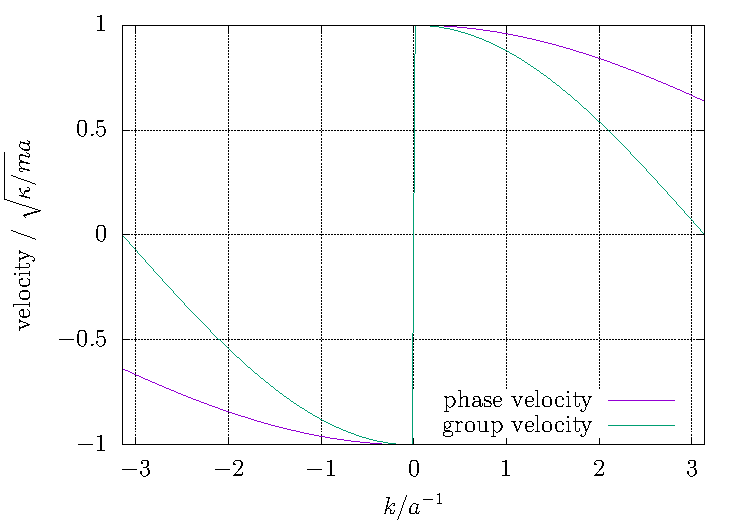
\includegraphics[width=.4\textwidth]{3-v-k.pdf}
            \caption{相速度$v_p$和群速度$v_g$关于波矢$k$的函数曲线图,其中横坐标$k$以$a^{-1}$为单位,纵坐标速度以$\sqrt{\frac{\kappa}{m}}a$为单位.}
            \label{3-v-k}
        \end{figure}
        \begin{itemize}
            \item[$\triangleright$] 声波的速度应当是波包移动的速度,故声速应当等于群速度,由于声波的波长很大,波矢$k$很小,在$k\rightarrow 0$的极限下,声速
            \begin{equation}
                \label{3-sound-velocity}
                v=\sqrt{\frac{\kappa}{m}}a.
            \end{equation}
            \item[$\triangleright$] 一维情况下压缩系数的定义为
            \begin{equation}
                \beta=-\frac{1}{L}\frac{\partial L}{\partial F},
            \end{equation}
            故有
            \begin{gather}
                \frac{1}{\beta}=-L\frac{\partial F}{\partial L}=-Na\frac{\partial F}{\partial(Na)}=-a\frac{\partial F}{\partial a}=-a\kappa,\\
                \Longrightarrow\kappa=-\frac{1}{a\beta}.
            \end{gather}
            一维原子链的线密度定义为
            \begin{equation}
                \rho=\frac{m}{a}.
            \end{equation}
            将上面两式代入式\eqref{3-sound-velocity}中可得
            \begin{equation}
                v=\sqrt{\frac{1}{\beta\rho}}.
            \end{equation}
        \end{itemize}
        \item[(e)] 单位角频率范围内的态密度为
        \begin{equation}
            g(\omega)=\frac{dN}{d\omega}=2\frac{dN}{dk}\frac{dk}{d\omega}=2\frac{dN}{dk}\frac{1}{v_g}.
        \end{equation}
        这里多出一个系数$2$,这是因为色散关系是关于$k$偶函数,一个$\omega$实际上对应着两个$k$.
        由于在周期性边界条件下
        \begin{equation}
            k=\frac{2n\pi}{L},\quad n=1,2,\cdot,N,
        \end{equation}
        相邻模式的$k$的间距均为$\frac{2\pi}{L}$,因此状态数是随着$k$均匀分布的,因此
        \begin{equation}
            \frac{dN}{dk}=\frac{N}{k}=\frac{L}{2\pi}=\frac{Na}{2\pi}.
        \end{equation}
        故单位角频率范围内的态密度为
        \begin{equation}
            g(\omega)=2\frac{Na}{2\pi}\sqrt{\frac{m}{\kappa}}\frac{1}{a}\frac{\abs{\sin(ak/2)}}{\sin(ak/2)}\frac{1}{\cos(ak/2)}=\frac{2N}{2\pi}\sqrt{\frac{m}{\kappa}}\frac{\abs{\sin(ak/2)}}{\sin(ak/2)}\frac{1}{\cos(ak/2)}.
        \end{equation}
        在第一布里渊区的右半边($0\leq k\leq \frac{\pi}{a}$),
        \begin{equation}
            g(\omega)=\frac{2N}{2\pi}\sqrt{\frac{m}{\kappa}}\frac{1}{\cos(ak/2)}=\frac{N}{\pi}\frac{1}{\sqrt{(\kappa/m)-(\omega/2)^2}}.
        \end{equation}
        \begin{itemize}
            \item[$\triangleright$] 态密度函数曲线如图\ref{3-g-omega}.
            \begin{figure}[h]
                \centering
                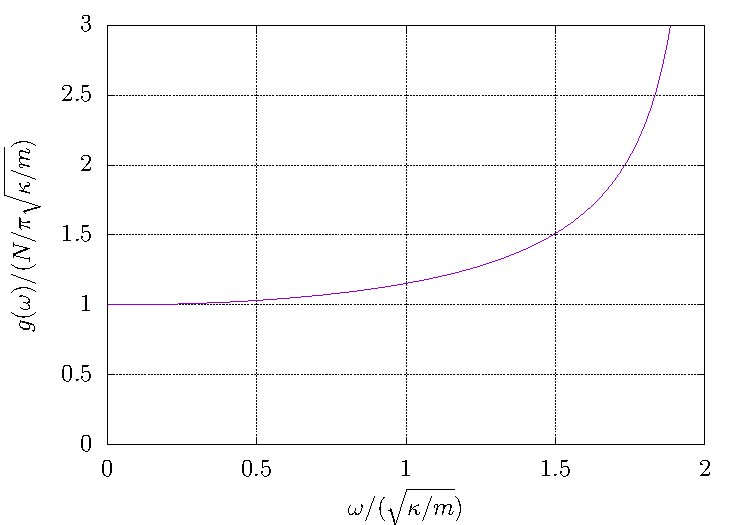
\includegraphics[width=.4\textwidth]{3-g-omega.pdf}
                \caption{单位角频率范围内的态密度,其中频率以$\sqrt{\kappa/m}$为单位,态密度$g(\omega)$以$\frac{N}{\pi\sqrt{\kappa/m}}$为单位.}
                \label{3-g-omega}
            \end{figure}
        \end{itemize}
        \item[(f)] 一维原子链的内能为
        \begin{equation}
            E=\int_0^{2\sqrt{\frac{\kappa}{m}}}d\omega\,g(\omega)\hbar\omega(n(\beta\hbar\omega)+\frac{1}{2})=\int_0^{2\sqrt{\frac{\kappa}{m}}}d\omega\,\frac{N}{\pi}\frac{\hbar\omega}{\sqrt{(\kappa/m)-(\omega/2)^2}}\left(\frac{1}{e^{\omega}-1}+\frac{1}{2}\right).
        \end{equation}
        一维原子链的热容为
        \begin{equation}
            C=\frac{\partial U}{\partial T}=\int_0^{2\sqrt{\frac{\kappa}{m}}}d\omega\,\frac{N}{\pi}\frac{\hbar\omega}{\sqrt{(\kappa/m)-(\omega/2)^2}}\frac{e^{\beta\hbar\omega}}{(e^{\beta\hbar\omega}-1)^2}\frac{\hbar\omega}{k_BT^2}.
        \end{equation}
        \item[(g)] 由于$\frac{x}{e^x-1}$可以展开为
        \begin{equation}
            \frac{x}{e^x-1}=1-\frac{x}{2}+\frac{x^2}{12}+\cdots,
        \end{equation}
        $n(\omega)+\frac{1}{2}$可以展开为
        \begin{equation}
            \label{3-EE}
            n(\omega)+\frac{1}{2}=\frac{1}{e^{\beta\hbar\omega}-1}+\frac{1}{2}=\frac{k_BT}{\hbar\omega}+\frac{1}{12}\frac{\hbar\omega}{k_BT}+\cdots
        \end{equation}
        在高温极限下,
        \begin{equation}
            n(\omega)+\frac{1}{2}=\frac{k_BT}{\hbar\omega}.
        \end{equation}
        一维原子链的热容为
        \begin{equation}
            C=\frac{\partial}{\partial T}\int_0^{2\sqrt{\frac{\kappa}{m}}}d\omega\,g(\omega)k_BT=k_BN.
        \end{equation}
        若保留式\eqref{3-EE}到第二项,
        \begin{equation}
            n(\omega)+\frac{1}{2}=\frac{k_BT}{\hbar\omega}+\frac{1}{12}\frac{\hbar\omega}{k_BT}.
        \end{equation}
        则热容为
        \begin{align}
            \nonumber C=&k_B+\frac{\partial}{\partial T}\int_0^{2\sqrt{\frac{\kappa}{m}}}d\omega\,\frac{N}{\pi}\frac{\hbar\omega}{\sqrt{(\kappa/m)-(\omega/2)^2}}\frac{1}{12}\frac{\hbar\omega}{k_BT}\\
            \nonumber=&k_B-\frac{N\hbar^2}{12\pi k_BT^2}\int_0^{2\sqrt{\kappa/m}}d\omega\,\frac{\omega^2}{\sqrt{(\kappa/m)-(\omega/2)^2}}\\
            \nonumber&(t=\omega/2\sqrt{\kappa/m})\\
            \nonumber=&k_B-\frac{N\hbar^2}{12\pi k_BT^2}8\frac{\kappa}{m}\int_0^{2\sqrt{\kappa/m}}dt\,\frac{t^2}{\sqrt{1-t^2}}\\
            \nonumber&(\sin\theta=t)\\
            \nonumber=&k_B-\frac{N\hbar^2}{12\pi k_BT^2}8\frac{\kappa}{m}\int_0^{\pi/2}d\theta\,\sin^2\theta\\
            \nonumber=&k_B-\frac{N\hbar^2\kappa}{6mk_B}\frac{1}{T^2}.
        \end{align}
        故
        \begin{equation}
            C/N=k_B(1-A/T^2+\cdots)
        \end{equation}
        其中
        \begin{equation}
            A=\frac{\hbar^2\kappa}{6mk_B^2}.
        \end{equation}
    \end{enumerate}
\end{sol}

\begin{prob}[(9.4) Decaying Waves]
    In the dispersion curve of the harmonic chain (Eq. 9.3), there is a maximum possible frequency of oscillation $\omega_{max}$. If a vibration with frequency $\omega>\omega_{max}$ is forced upon the chain (say by a driving force) the "wave" will not propagate along the chain, but rather will decay as one moves away from the point where the oscillation is imposed (this is sometimes known as an "evanescent" wave). With $\omega>\omega_{max}$ solve Eq. 9.3 for a complex $k$ to determine the decay length of this evanescent wave. What happens to this length as $\omega\rightarrow\omega_{max}$?
\end{prob}
\begin{sol}
    由式(9.3)
    \[
        \omega=2\sqrt{\frac{\kappa}{m}}\abs{\sin\left(\frac{ak}{2}\right)},
    \]
    最大的可能频率为
    \begin{equation}
        \omega_{max}=2\sqrt{\frac{\kappa}{m}}.
    \end{equation}
    求解式(9.3):
    \begin{gather}
        \omega=2\sqrt{\frac{\kappa}{m}}\abs{\sin\left(\frac{ak}{2}\right)}=2\sqrt{\frac{\kappa}{m}}\sqrt{\frac{1-\cos(ak)}{2}}\\
        \Longrightarrow\omega^2=2\frac{\kappa}{m}(1-\cos(ak))\\
        \Longrightarrow k=a^{-1}\arccos\left(1-\frac{m\omega^2}{2\kappa}\right).
    \end{gather}
    利用
    \begin{equation}
        \arccos(z)=-i\ln(z+\sqrt{z^2-1}),
    \end{equation}
    有
    \begin{equation}
        k=-ia^{-1}\ln\left[1-\frac{m\omega^2}{2\kappa}+\sqrt{-\frac{m\omega^2}{\kappa}+\frac{m^2\omega^4}{4\kappa}}\right]
    \end{equation}
    注意到当$\omega>\omega_{max}$时,上面中括号内为负的实数,利用
    \begin{equation}
        \ln z=\ln\abs{z}+i\arg z,
    \end{equation}
    有
    \begin{equation}
        k=\frac{\pi}{a}-ia^{-1}\ln\left[\frac{m\omega^2}{2\kappa}-\sqrt{-\frac{m\omega^2}{\kappa}+\frac{m^2\omega^4}{4\kappa}}\right].
    \end{equation}
    故这一衰减波的衰减距离为
    \begin{equation}
        -\text{Im}(k)^{-1}=\frac{a}{\ln\left[\frac{m\omega^2}{2\kappa}-\sqrt{-\frac{m\omega^2}{\kappa}+\frac{m^2\omega^4}{4\kappa}}\right]}.
    \end{equation}
    当$\omega\rightarrow\omega_{max}$时,
    \begin{equation}
        -\text{Im}(k)^{-1}\rightarrow+\infty.
    \end{equation}
    衰减距离变为无穷大.
\end{sol}

\begin{prob}[(9.7) General Proof That Normal Modes Become Quantum Eigenstates$^*$]
    This proof generalizes the argument given in Exercise 9.1. Consider a set of $N$ particles $a=1,\dots,N$ with mass $m_a$ interacting via a potential
    \[
        U=\frac{1}{2}\sum_{a,b}x_aV_{a,b}x_b
    \]
    where $x_a$ is the deviation of the position of particle $a$ from its equilibrium position and $V$ can be taken (without loss of generality) to be symmetric matrix. (Here we consider a situation in 1d, however, we wil see that to go to 3d we just need to keep track of three times as many coordinates.)
    \begin{itemize}
        \item[i.] Defining $y_a=\sqrt{m_a}x_a$, show that the classical equations of motion may be written as
        \[
            \ddot{y}_a=-\sum_bS_{a,b}y_b
        \]
        where
        \[
            S_{a,b}=\frac{1}{m_a}V_{a,b}\frac{1}{\sqrt{m_b}}
        \]
        Thus show that the solutions are
        \[
            y_a^{(m)}=e^{-i\omega_mt}s_a^{(m)}
        \]
        where $\omega_m^2$ is the $m^{th}$ eigenvalue of the matrix $S$ with corresponding eigenvector $s_a^{(m)}$. These are the $N$ normal modes of the system.
        \item[ii.] Recall the orthogonality relation for eigenvectors of hermitian matrices
        \begin{gather}
            \sum_a[s_a^{(m)}]^*[s_a^{(n)}]=\delta_{m,n}\tag{9.8}\\
            \sum_m[s_a^{(m)}]^*[s_b^{(m)}]=\delta_{a,b}\tag{9.9}
        \end{gather}
        Since $S$ is symmetric as well as hermitian, the eigenvectors can be taken to be real. Construct the transformed coordinates
        \begin{gather}
            Y^{(m)}=\sum_as_a^{(m)}x_a\sqrt{m_a}\tag{9.10}\\
            P^{(m)}=\sum_as_a^{(m)}p_a/\sqrt{m_a}\tag{9.11}
        \end{gather}
        show that these coordinates have canonical commutations
        \[
            [P^{(m)},Y^{(n)}]=-i\hbar\delta_{n,m}\tag{9.12}
        \]
        and show that in terms of these new coordinates the Hamiltonian is rewritten as
        \[
            H=\sum_m\left[\frac{1}{2}[P^{(m)}]^2+\frac{1}{2}\omega_m^2[Y^{(m)}]^2\right]
        \]
        Conclude that the quantum eigenfrequencies of the system are also $\omega_m$. (Can you derive this result from the prior two equations?)
    \end{itemize}
\end{prob}
\begin{sol}
    \begin{enumerate}
        \item[i.] 第$a$个粒子受力
        \begin{equation}
            F_a=-\frac{\partial U}{\partial x_a}=-\sum_bV_{a,b}x_b-V_{a,a}
        \end{equation}
        由于一维原子链中原子数很多,$N\gg 1$,故上式可近似为
        \begin{equation}
            F_a\approx-\sum_bV_{a,b}x_b=\sum_bS_{a,b}\frac{y_b}{\sqrt{m_b}}.
        \end{equation}
        第$a$个粒子的经典运动方程为
        \begin{gather}
            m_a\ddot{x}_a=F_a\\
            \Longrightarrow\ddot{y}_a=-\sum_bS_{a,b}y_b,
        \end{gather}
        其中
        \begin{equation}
            S_{a,b}=\frac{1}{\sqrt{m}_a}V_{a,b}\frac{1}{\sqrt{m_b}}.
        \end{equation}
        上面的经典运动方程化为线性代数形式为
        \begin{equation}
            \label{5-ME-L}
            \frac{d^2}{dt^2}y=-Sy.
        \end{equation}
        设解为
        \begin{equation}
            y_a=s_ae^{i\omega t}.
        \end{equation}
        代入式\eqref{5-ME-L}得
        \begin{equation}
            -\omega^2y=-Sy.
        \end{equation}
        据题设$\omega_m^2$为$S$的本征值,故
        \begin{equation}
            y_a^{(m)}=e^{-i\omega_mt}s_a^{(m)}.
        \end{equation}
        \item[ii.] 如题设
        \begin{align}
            Y^{(m)}=&\sum_as_a^{(m)}x_a\sqrt{m_a},\\
            P^{(m)}=&\sum_as_a^{(m)}p_a/\sqrt{m_a}.
        \end{align}
        $P^{m}$和$Y^{(n)}$的对易关系为
        \begin{align}
            \nonumber[P^{(m)},Y^{(n)}]=&[\sum_as_a^{(m)}x_a\sqrt{m_a},\sum_bs_b^{(m)}p_b/\sqrt{m_b}]\\
            \nonumber=&\sum_a\sum_bs_a^{(m)}s_b^{(n)}[x_a,p_b]\\
            \nonumber=&\sum_a\sum_bs_a^{(m)}s_b^{(n)}(-i\hbar\delta_{a,b})\\
            \nonumber=&-i\hbar\sum_as_a^{(m)}s_a^{(n)}\\
            =&-i\hbar\delta_{mn}.
        \end{align}
        系统的哈密顿为
        \begin{equation}
            H=\sum_a\frac{p_a^2}{2m_a}+U=\sum_a\frac{p_a^2}{2m_a}+\frac{1}{2}\sum_{a,b}x_aV_{a,b}x_b.
        \end{equation}
        由于
        \begin{align}
            \nonumber\sum_m\frac{1}{2}[P^{(m)}]^2=&\frac{1}{2}\sum_m\left(\sum_as_a^{(m)}p_a/\sqrt{m_a}\right)\left(\sum_bs_b^{(m)}p_b/\sqrt{m_b}\right)\\
            \nonumber=&\frac{1}{2}\sum_a\sum_b\frac{p_ap_b}{\sqrt{m_am_b}}\sum_ms_a^{(m)}s_b^{(m)}\\
            \nonumber=&\frac{1}{2}\sum_a\sum_b\frac{p_ap_b}{\sqrt{m_am_b}}\delta_{a,b}\\
            =&\sum_a\frac{p_a^2}{2m_a}.
        \end{align}
        以及
        \begin{align}
            \nonumber\frac{1}{2}\sum_m\omega_m^2[Y^{(m)}]^2=&\frac{1}{2}\sum_m\omega_m\left(\sum_as_a^{(m)}x_a\sqrt{m_a}\right)\left(\sum_bs_b^{(m)}x_b\sqrt{m_b}\right)\\
            \nonumber=&\frac{1}{2}\sum_a\sum_b\sqrt{m_am_b}x_ax_b\sum_ms_a^{(m)}\omega_m^2s_b^{(m)}\\
            \nonumber=&\frac{1}{2}\sum_a\sum_b\sqrt{m_am_b}x_ax_b\sum_ms_a^{(m)}\left(\sum_cS_{b,c}s_c^{(m)}\right)\\
            \nonumber=&\frac{1}{2}\sum_a\sum_b\sum_c\frac{\sqrt{m_am_b}}{\sqrt{m_bm_c}}\sum_ms_a^{(m)}V_{b,c}s_c^{(m)}\\
            \nonumber=&\frac{1}{2}\sum_a\sum_b\sum_c\frac{\sqrt{m_a}}{\sqrt{m_c}}x_aV_{b,c}x_b\delta_{a,c}\\
            \nonumber=&\frac{1}{2}\sum_a\sum_bx_bV_{b,a}x_a=U.
        \end{align}
        (注意由于$s_a^{(m)}$是实数,$[s_a^{(m)}]^*=[s_a^{(m)}]$.)故系统的哈密顿可表为
        \begin{equation}
            H=\sum_m\left[\frac{1}{2}[P^{(m)}]^2+\frac{1}{2}\omega_m^2[Y^{(m)}]^2\right].
        \end{equation}
        这相当于是多个简谐振子哈密顿的和,每个简谐振子的本征频率为$\omega_m$.
    \end{enumerate}
\end{sol}
\end{document}